\section{Related Work}
\label{sec:related}

The technologies based on DNNs have been used widely in data science, since DNNs have shown great promise in image recognition~\cite{krizhevsky2012imagenet}.
Also, a number of researchers have proposed new models beyond the state-of-the-art techniques.
In this section we introduce some previous studies related to this work.
We discuss how visualizations have played in development of DNN models and the differences between our work and the previous work.

% \subsection{Visualization in Deep Learning}
Although DNNs make great achievements, understanding of what computations performed at intermediate layers of DNNs is still limited.
Some previous studies have developed tools that help understand the processes in DNNs through visualization techniques.
They have proved such tools can help DNN developers improve their network models~\cite{tzeng2005opening,yosinski2015understanding,liu2017towards}.
Here, we discuss the roles of visualization with regard to the following three topics:

\textbf{Understanding of the Underlying Processes in Networks:}
The most important purpose of visualizations for DNNs is to understand the underlying processes in networks.
The visualizations can be classified into two categories according to which aspects of the network are visualized: \textbf{Inner Process} and \textbf{Learned Features}.
\begin{itemize}
\item \textbf{Inner Process:}
Visualizations in this category directly represent the interactions between neurons in a network.
These visualizations enable intuitive understanding of the inner processes in the networks.
Tzeng and Ma~\cite{tzeng2005opening} employed a directed acyclic graph (DAG) to show the interactions between neurons in the three different layers: input, hidden, and output.
The visualization, however, has a visual clutter issue when handling a large number of neurons.
Liu et al.~\cite{liu2017towards} also used a similar type of visualization, but they mitigate the issue.
They clustered layers and neurons in networks, selected representative layers and neurons, and illustrated those by a hybrid visualization.
Harley~\cite{harley2015interactive} developed an interactive and intuitive visualization system for DNNs.
Given an input image drawn by an user, the visualization system shows not only the features learned by networks, but also the behavior (i.e., activation and interaction) of neurons and layers.

\item \textbf{Learned Features:}
This type of visualizations focuses on visualizing the features learned by networks rather than the behavior in networks.
Since Convolutional Neural Networks (CNNs), a specific type of DNNs, have been widely used for image classification, many visualization approaches have been proposed to understand how images are classified by CNNs~\cite{erhan2009visualizing,zeiler2014visualizing,yosinski2015understanding,nguyen2016multifaceted}.
The visualizations display synthetic images produced by gradient-based techniques including deconvolution, code inversion, activation maximization\textemdash these techniques are based on high activations (learned features) of neurons of a network.
The images (although they do not look natural) would provide insight into the network model and can suggest potential directions to improve the model.
In addition to CNNs, Recurrent Neural Networks (RNNs) are getting attention since RNNs have achieved a great performance for sequential data, such as streaming, speech, and document.
Strobelt~\cite{strobelt2016visual} proposed a visual analytics system to understand a RNN-based model, where the system helps users explore hidden states in RNNs and find similar patterns in data.
\end{itemize}

The previous studies have made great achievements and shown the importance of visualization in development of DNNs.
However, they still have limitations.
For the clustering approach, when handling a large network, finding an appropriate abstraction level of networks would be a challenge.
Also, the DAG-based visualizations have a limitation in supporting other types of networks beside CNN-based networks.
For visualizing learned features, when the number of samples and classes is huge, it would be not easy to gain insights into the networks by analyzing the learned features of every single samples.
Although our approach is close to the second category, we focus on visualizing and understanding classification results of any types of DNNs.
%We argue that after DNN developers gain insights into data and classification results, they would more effectively understand the inner processes and the learned features using the aforementioned techniques than without the initial step.

% We argue that it should be effective to improve a network model after understanding initial classification results by using a basic network model.
% For classification tasks in real industrial world applications, such as medical records, CT scan images, 2D neutron scattering images, those who develop DNNs for a specific application would be not experts in the area.
% Therefore, in the situation that DNN developers has no background knowledge about the data they are dealing with and cannot expect the output, starting with the understanding of initial classification outputs resulted by their prototype model should help them develop the model for a specific data.
% After this preceding step, they would more effectively understand the inner processes and the learned features using the aforementioned techniques than without the step.

\textbf{Visualization for Classification Result:}
Visualization enables a better understanding of the classification results of neural networks.
Especially, when handling a large size of samples, suitable visualization techniques are required.
Most techniques have used a 2D-embedding type of visualization (Figure~\ref{fig:t-sne}) to represent the classification results.
An output layer of neural networks usually produce predicted scores for each sample across all classes.
They project the prediction scores on a 2D space by dimensionality reduction techniques, such as t-SNE, PCA, etc~\cite{maaten2008visualizing,rauber2017visualizing,kahng2018activis,paiva2015approach}.
This type of visualizations has a visual clutter issue caused by the large number of data points.
If the number of classes is large, the issue will become even worse.
Also, the visualizations are not able to reveal the assigned predicted score distribution over the classes.
Our visual representation solves these issues.
Our stripe visualization has a better scalability, resolves the visual clutter issue, and effectively shows the probability distribution by integrating a parallel coordinated visualization into our tool.
Details are described in Section~\ref{sec:visualization}.
Ren et al.~\cite{ren2017squares} proposed a visualization for performance analysis in machine learning.
Their major visual metaphor and the way they use that metaphor is similar to our approach.
In this paper, our visualization tool focuses on the understanding of classification results rather than performance analysis.
Besides, we visualize how the outcome changes, which samples are continuously misclassified, and what features are learned by the neural networks as the training progress.
This provides opportunities to improve the model.

\textbf{Direct Manipulation:} Few previous studies proposed approaches that support direct manipulation of neural networks and a real-time visualization of the networks~\cite{smilkov2016direct,chung2016revacnn}.
Both Playground~\cite{smilkov2016direct} and ReVACNN~\cite{chung2016revacnn} provide similar features.
They support real-time visualization of how neural networks are trained and real-time model steering\textemdash selecting filters, adding/removing neurons/layers, and adjusting weights.
The tools help users gain an intuition about deep neural networks.
Playground, however, is designed for an educational purpose rather than real-world applications.

\begin{figure}[tb]
\centering
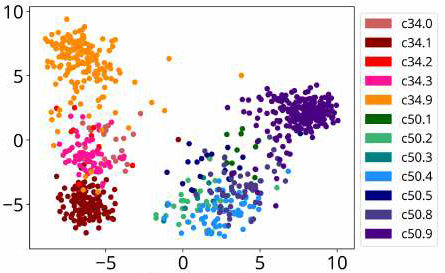
\includegraphics[width=0.7\columnwidth]{2d-embedding}
\caption{
2D-embedding of cancer pathology reports using PCA.
The colors of the points denote their classes.
%This type of visualization has limitations in understanding a classification result~\cite{rauber2017visualizing}.
}
\label{fig:t-sne}
%\vspace{-0.8cm}
\end{figure}


% \item Visualizing the Hidden Activity of Artificial Neural Networks~\cite{rauber2017visualizing}
% \item Recurrent Models of Visual Attention
% \item VISUALIZING AND UNDERSTANDING RECURRENT NETWORKS
% \item Towards Transparent AI Systems: Interpreting Visual Question Answering Models
% \item ML-o-scope: a diagnostic visualization system for deep machine learning pipelines
% \item Visualizing Deep Convolutional Neural Networks Using Natural Pre-imag
% Increase Transparency - Interpreting Black-Box Classifiers Using Instance-Level Visual Explanations

% \subsection{Visualization for Classification}

% \begin{enumerate}
% \item Modelling, Visualising and Summarising Documents with a Single Convolutional Neural Network
% \item Convolutional Neural Networks for Sentence Classification
% \item Power to the People: The Role of Humans in Interactive Machine Learning
% \item Visualizing and Understanding Neural Models in NLP
% \item Multi-task Deep Neural Networks for Automated Extraction of Primary Site and Laterality Information from Cancer Pathology Reports~\cite{yoon2016multi}
% \end{enumerate}